%!TEX root = ThesisLKN.tex
\chapter{Results and Discussions} \label{chapter:5}


\section{Metrics} \label{sec:metrics}

\subsection{Metrics for Neural Network}

\subsection{Metrics for Tracking}

The possible metrics that could be used for measuring the consistency between occupancy predicition and ground truth are: \textit{cross entropy}, \textit{f1 score} and \textit{average precision}.  We choose average precision as our metric and the reasons will be detailed in the thesis.

\section{Training of Neural Network}

After the data is collected as described in Section \ref{sec:traj_sim}, we split them into training, validation and test set. The training and validation set are sampled from seven full maps, and test set is sampled from a separate map. The number of samples we generated are summarized in Table \ref{table:nos}. 

Figure \ref{fig:trajs} shows one example of map window as network input and its ground truth. On the left, a cell is labeled with red color, and the sampled trajectories that go through this cell are displayed. On the right, it shows a visualization of the ground truth \( P_c(V^{ex} | V^{en}) \) for that red cell. The axes show velocities on \( x, y\) directions. Since we assume a person has maximum speed of 1 $cell/timestep$, the velocities must be in range $[-1,1]. $Outer axes represent entering direction \( V^{en} \), and inner represents exit velocity \( V^{ex} \). One can see that \( P(V^{ex}=DL | V^{en}=DL) = 0.13 \) and \( P(V^{ex}=D | V^{en}=DL) = 0.87 \) \footnote{DL represents going down-left, and its corresponding velocity is (-1, -1). D represents going down, and its velocity is (0, -1).}. This indicates that if a person reaches the red cell by taking direction down-left (i.e., coming from upper-right neighboring cell), it is very likely that he or she will change to going down for the next time step. This proves that our way of modeling motion pattern captures human motion dynamics.

\begin{table}[t]
\centering
  \begin{tabular}{c|ccc}
    \hline
     & training & validation & test \\ \hline
    number of samples & 27,119 & 4,785 & 3,760\\
    \hline
  \end{tabular}
\caption{Number of samples in training, validation and test set.}
\label{table:nos}
\end{table}

\begin{figure}[H]
\begin{tabular}{ll}
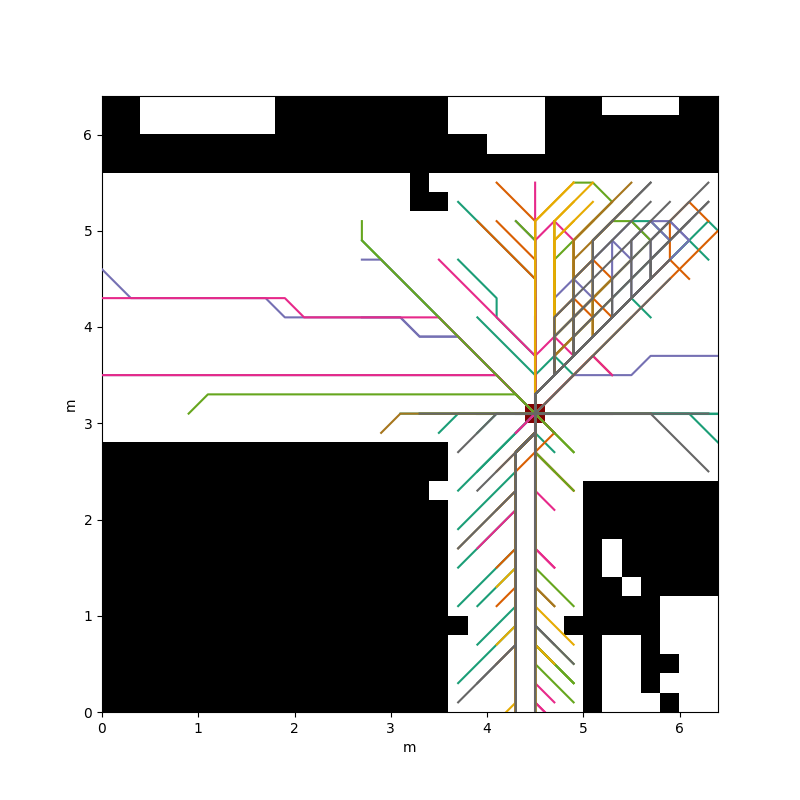
\includegraphics[width=0.48\textwidth]{figures/trajs_through_cell.png}
&
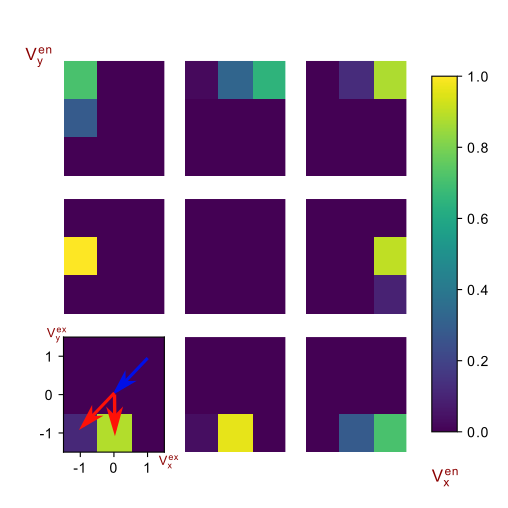
\includegraphics[width=0.48\textwidth]{figures/probs_on_that_cell_2.png}
\end{tabular}
\caption[one example of map window as network input and its ground truth]{one example of map window as network input and its ground truth \textbf{Left}: The map window has size of \( 32 \times 32 \) cells, with resolution of \( 0.2m/cell\). It also shows trajectories that goes through the red cell. \textbf{Right}: Visualization of conditional probability \( P_c(V^{ex} | V^{en}) \) for the red cell on left map. It can be seen that if a person reaches that cell by taking down-left direction, it is very like that he or she will change direction to going down.}. 
\label{fig:trajs}
\end{figure}

\begin{figure}[ht]
  \centering
    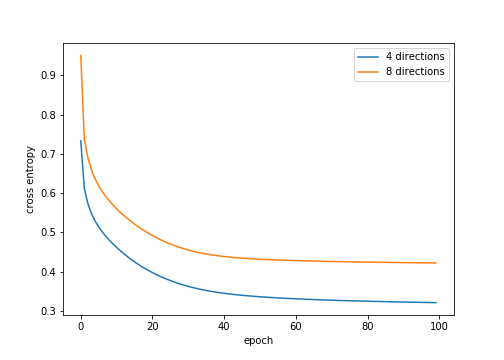
\includegraphics[width=.7\textwidth]{figures/training_hist.png}
    \caption{Cross entropy loss during training. The networks are trained to learn conditional probabilities \( P_c(V^{ex} | V^{en}) \). The blue line shows training dynamics using data generated with 4 directions "left, right, up and down". The yellow line also takes diagonal directions into account, which has 8 directions in total. }
    \label{fig:trainning}
\end{figure}

Practically, the hyperparameters of a neural network, such as learning rate and weight decay, are optimized by random search. However, due to time limitation, this step is skipped in this thesis work. Instead, we use the hyperparamters from a similar network (the only difference is the output layer) that is optimized for predicting average human occupancy on static map. The network is trained with mini-batches of size of 128, and  is optimized with Adam optimizer \citep{Kingma2014Adam}. The training runs for 100 epochs, with early stopping patience of 15 epochs. The best model is selected based on the KL-divergence on validation data.

 Figure \ref{fig:trainning} shows the cross entropy loss during training. We trained networks for two cases: 4 directions and 8 directions. The 4-direction case considers only "left, right, up and down". Therefore, the dimension of its output is $32 \times 32 \times 16$. The 8-direction case considers also diagonal directions, therefore the output dimension is $32 \times 32 \times 64$. The loss curves show that the hyperparameters are set correctly since the loss decreases exponentially in the early stage and keeps decreasing afterwards. Naturally, more directions implies higher complexity, thus the overall loss for yellow line is higher than blue line. The cross entropy on the test set is listed in Table \ref{table:loss_on_test}.

 \begin{table}[H]
\centering
  \begin{tabular}{c|c}
    \hline
     networks      &      cross entropy  \\ \hline
     4-direction   &      0.334 \\ \hline
     8-direction   &      0.383 \\          
   \hline
 \end{tabular}
\caption{Cross entropy loss on test data.}
\label{table:loss_on_test}
\end{table}

\section{Evaluation of Tracking Performance}

Our method BOFMP is proposed for human tracking in indoor environment. It is similar to BOFUM, and we claim it improves BOFUM since it is able to predict occupancy according to human motion pattern. To verify our claim, we compare the performance of BOFUM and BOFMP in two scenarios:

\begin{my_enumerate}
\item \textbf{tracking stage}. Before a certain time point \( t_{lost} \), measurements are given at each time step, i.e., $t=1:t_{lost}-1$. We evaluate consistency between occupancy prediction and the ground truth at every time step.
\item \textbf{future prediction stage}. From time point \( t_{lost} \) on, the measurement is no longer given. Then we evaluate occupancy predictions with ground truth for the next \( n \) time steps.
\end{my_enumerate}

These two stages can be illustrated as:
\[\text{start} \rightarrow \text{tracking stage} \xrightarrow{\text{measurement lost}} \text{future prediction stage} \rightarrow \text{end}\]
In this thesis, we set $t_{lost}=9$ and $n=8$, i.e., both tracking and future prediction stage lasts for 8 time steps. The parameters of filters are tuned based on their performance in \textit{future predictions} stage. 

  % The measurement is lost at time step \( t=9\), and we select the best set of parameters based on the average of average precisions for the next \( 8 \) time steps. 

\subsection{Overview of Datasets}

\textbf{Simulated Dataset}

We generated 500 scenes as training set for tuning filter parameters and 500 scenes for test set. Training and test data are generated from different maps. In these scenes, there are either one or two walking humans. Two examples of scenes in training set are shown in Figure \ref{fig:sample_scene_simulated}.

\begin{figure}[hp]
  \centering
  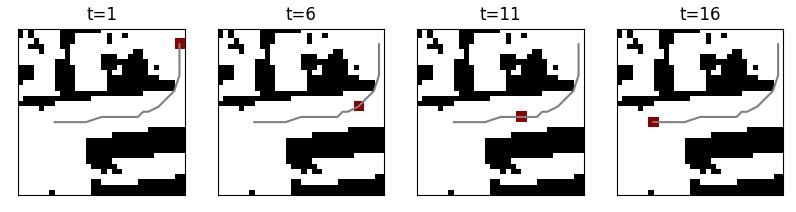
\includegraphics[width=.99\textwidth]{figures/simulated_dataset_1_persons_with_traj.png}
    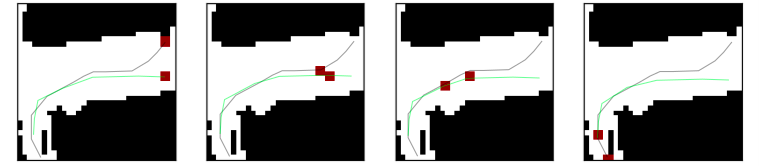
\includegraphics[width=\textwidth]{figures/simulated_dataset_2_persons_with_traj.png}
    \caption[Two examples of scenes in simulated training set.]{Two examples of scenes in simulated training set. Each person is indicated by a red square and the lines show the trajectory for each person. \textbf{Up}: This example shows a person firstly make a turn and then go straight along the corridor. \textbf{Down}: Two persons are walking in the map window with different speed. Clearly, the one the gray trajectory has a higher speed than the one with green trajectory.}
    \label{fig:sample_scene_simulated}

    \vspace*{\floatsep}

    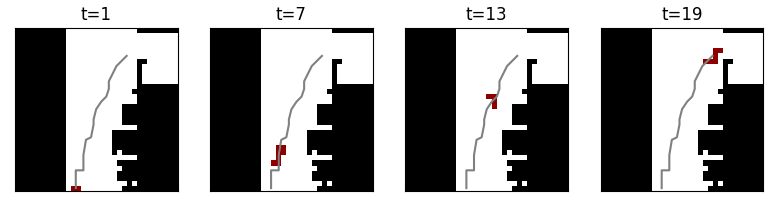
\includegraphics[width=.98\textwidth]{figures/real_dataset_1_persons_1_crop.png}
    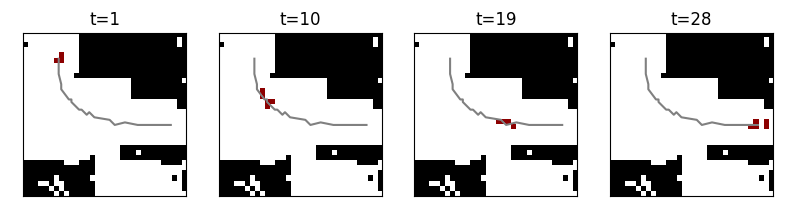
\includegraphics[width=\textwidth]{figures/real_dataset_1_persons_crop.png}
    \caption[Two examples of scenes in real training set.]{Two examples of scenes in real training set. \textbf{Up}: This example shows a person going from bottom towards the door in the upper right corner. \textbf{Down}: It shows a person is making a turn. }
    \label{fig:sample_scene_real}


\end{figure}


\textbf{Real Dataset}

Although our neural network are trained on simulated human trajectories, we expect that our method outperforms BOFUM on real tracking scenes. We record human trajectories on two different maps by a laser scanner mounted on a robot. After processing raw laser data, we get 500 tracking scenes for training from one of the maps and 244 scenes for test from the other. Figure \ref{fig:sample_scene_real} shows twos examples of scenes in training set.

\subsection{Tracking on Simulated Data}

For both filters, we randomly sample 100 sets of parameters from value ranges listed in Table \ref{table:param_range_simulated}, apply them on scenes in the training set and calculate average precision for every time step. The best set of parameters for each filter are selected based on the mean of average precision in the future prediction stage. 

\begin{table}[H]
\centering
  \begin{tabular}{c|c}
    \hline
     &   value range for simulated data \\ \hline
    \( e \) & \( \{3, 5, 7\} \) \\
    \(  \delta^2\) & \( [0.1, 0.6]\) \\   
   \( \Omega \) & \( [0.01, 0.2] \) \\
   \hline
 \end{tabular}
\caption{Value ranges of filter parameters for simulated data.}
\label{table:param_range_simulated}
\end{table}

 We firstly tuned the parameters on training set for BOFUM and BOFMP individually. Then we apply both filters with their best parameters on test set. The best set of parameters and its corresponding average precision from \( t=9 \) to \( t=16 \) on test data are listed in Table \ref{table:best_param_simulated}. 

\begin{table}[H]
\centering  
\begin{tabularx}{\textwidth}{c|c|c|c|c|c}
    \hline
    & $ e $ & $ \delta^2 $ & $ \Omega $ & average precision for $t=8:16 $ & mean\\ \hline
    BOFUM & 7 & 0.556 & 0.0164 &  0.767  0.599  0.500    0.416  0.349  0.279  0.232  0.192 & 0.417 \\
    BOFMP & 7 & 0.373 & 0.0353 & 0.785  0.637  0.552  0.479  0.416  0.358  0.311  0.252 & 0.474 \\
   \hline
  \end{tabularx}
\caption{Best parameters for BOFUM and BOFMP on simulated data.}
\label{table:best_param_simulated}
\end{table}

Figure \ref{fig:simulated_test_data} shows mean of average precision on 500 scenes in test set for every time step. The average precision for both filters start with values close to zero. Since we highly trust our measurements (low $\Omega$), both filters are able to successfully track the objects within 3 time steps. The fact that average precision keeps a high value from $t=3$ to $t=8$ indicates that both filters can predict very well for the \textit{next immediate} time step. Starting from $t=9$ (see the red dash line), measurements are no longer given. The prediction is still accurate for the next time step ($t=9$), but decreases progressively over time.  This is expected, since without measurements, the state of world becomes more and more uncertain. Even though, we can see that our BOFMP have a higher average precision value than BOFUM at almost every time step, which indicates the improvements of our method in both tracking and future prediction stages.

Figure \ref{fig:tracking_simulated_data} shows how BOFUM and BOFMP perform tracking on one scene from test data. In this example, a person is walking from the lower door towards upper door. The gray curve shows the trajectory of the person. At $t=8$, the person walks upwards with velocity of 1 $cell/timestep$. Both algorithms track the person very well with average precision of $1.0$. At $t=9$, the measurement is lost and the future prediction stage of tracking starts. At $t=10$, BOFUM predicts that the person will continue to go upwards, with a low possibility going other directions. However, since BOFMP knows there is a door in the top right corner, it predicts that the person is also very likely going to that door, and thus turns to upper right. At later time steps, BOFMP continues to predict occupancy towards upper door as well as other possible directions (i.e., door on the left and empty space on the right). On the contrary, BOFUM still propagates most occupancies upwards. At $t=16$, since the object accelerates to higher velocity, most of occupancy predictions of BOFMP are left behind the tracking object.

\begin{figure}[hp]
  \centering
    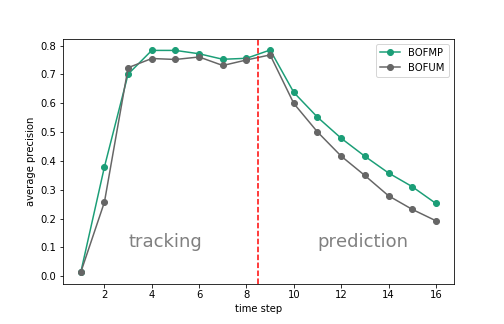
\includegraphics[width=.8\textwidth]{figures/test_on_simulated_data.png}
    \caption[Evaluation results on simulated test data.]{Evaluation results on simulated test data. The tracking stage lasts from $t=1:8$, and future prediction starts from $t=9$. One can see that in both stages, our proposed BOFMP outperforms BOFUM for almost every time step.}
    \label{fig:simulated_test_data}
\end{figure}

\begin{figure}[H]
  \centering
    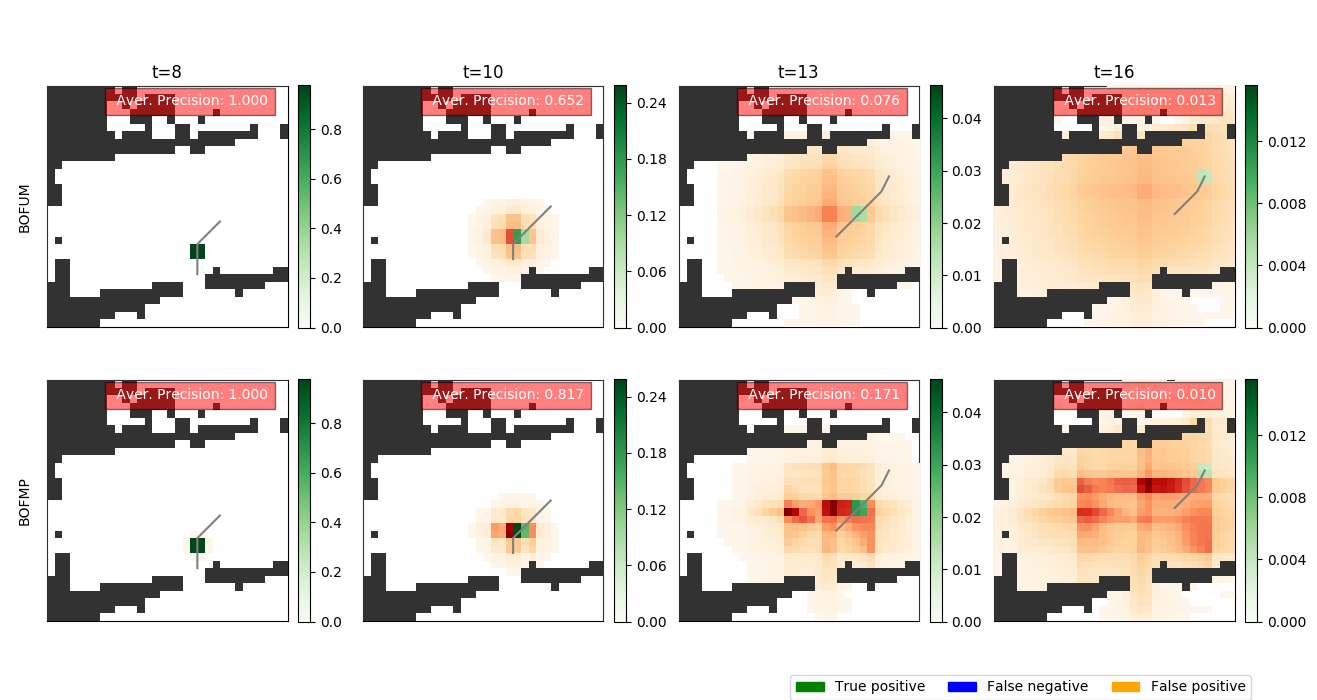
\includegraphics[width=\textwidth]{figures/tracking_sample_for_simulated_data.png}
    \caption{One example of tracking case from test data. A person is walking from the lower door to the door in the upper right corner. The measurement is lost at $t=9$. For BOFUM, it predicts most occupancies going upwards. For our BOFMP, since it has knowledge on the human motion model, it predicts occupancies to all possible directions, such as going to the door in the upper right corner, the door on the left and empty space on the right.}
    \label{fig:tracking_simulated_data}
\end{figure}

\subsection{On real data}

Table \ref{table:param_range_real} shows the value ranges from which the filter parameters are sampled. Note that value range of noise variance $\delta^2$ for real data is higher than that for simulated data. This is because in real data, there are higher uncertainties with human motion and sensor failures.

\begin{table}[H]
\centering
  \begin{tabular}{c|c|}
    \hline
     &  value range for real data \\ \hline
    \( e \) &  \( \{3, 5, 7\} \)\\
    \(  \delta^2\) & \( [0.2, 0.7]\) \\   
   \( \Omega \) & \( [0.01, 0.2] \)\\
   \hline
 \end{tabular}
\caption{Value ranges for filter parameters on real data.}
\label{table:param_range_real}
\end{table}

\textbf{Spatial blurring of motion probabilities}

The simulated trajectories do not always reflect real human motion patterns. This is because, as shown in Figure \ref{fig:blur_idea}, people are more flexible to decide when and where to make turns. 

\begin{figure}[ht]
  \centering
   \captionsetup{width=\linewidth}
    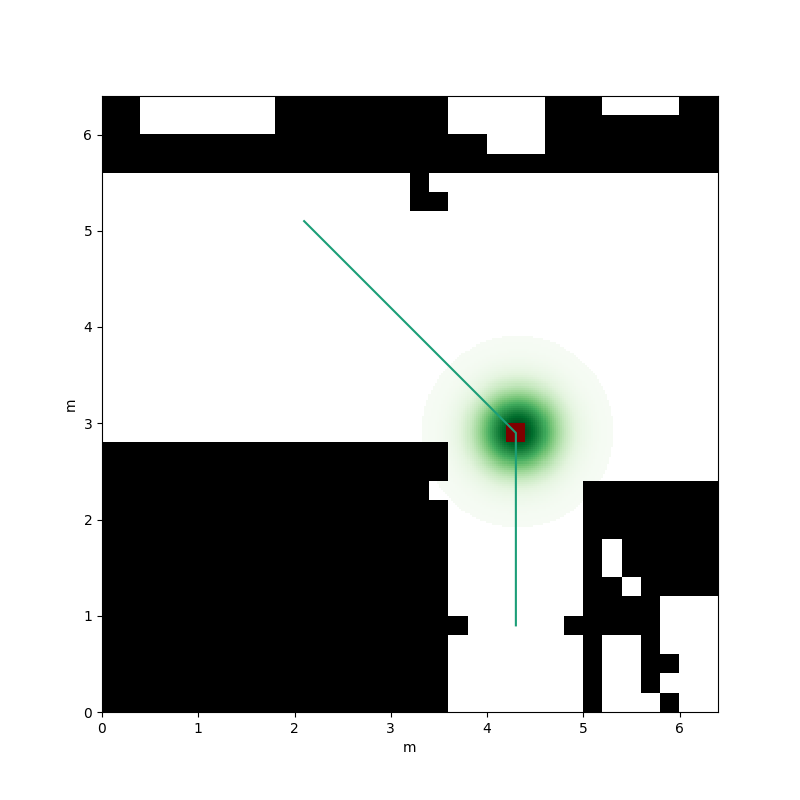
\includegraphics[width=.6\textwidth]{figures/blur_idea.png}
    \caption{A turn on simulated human trajectory. In order to reach the goal location in upper left corner, the simulated trajectory shows that a person will make a turn from going up to going up-left at location indicated by the red square. However, in real scenarios, a person is more flexible in deciding where to make that turn and he might turn at any location in the green area.}
    \label{fig:blur_idea}
\end{figure}

Therefore, to better adapt to real data, we introduce a technique that blurs the motion pattern probabilities  \( P_c(V^{ex} | V^{en}=v\} \) of a cell $c$ \textit{spatially} into its neighbors if a \textit{turn} is detected. A \textit{turn} on cell $c$ for velocity $v^{en}$ is defined as:

\[ 
turn(c, v^{en}) = 
\begin{cases}
    True , &  \argmax_v (P_c(V^{ex}=v | V^{en}=v^{en}) \, \neq \, v^{en} \\
    False,              & \text{otherwise}
\end{cases}
 \]


For each detected turn at cell $c$, we add its motion probability $P_c(V^{ex} | V^{en}=v^{en})$ to that of its neighboring cells in a Gaussian blurring way. Intuitively, this means if a person makes a turn at a certain cell, it is also likely that people make that turn somewhere near that cell. As a consequence, another two parameters, blur extent \( blurExt \) and blur variance  \( blurVar \), are introduced and their value ranges are listed in Table \ref{table:spatial_blur_param_range}. If a turn is detected on cell $c$ for velocity $v^{en}$, for its neighboring cell $n$ that is less than $blurExt$ cells away from $c$,
\begin{equation}
P_n(\cdot| v^{en}) = P_n(\cdot| v^{en})  + P_c(\cdot| v^{en}) \times G(pos(n)-pos(c))
\end{equation}
where $G \sim \mathcal{N}(\mathbf{0}, \Sigma)$ is a 2-dimensional discrete Gaussian kernel.
\begin{table}[H]
\centering  
\begin{tabularx}{.8\textwidth}{c|c|c}
    \hline
      &  \textit{value range } & \textit{note} \\ \hline
    \( blurExt \) & \( \{3, 5, 7, 9\} \) & \footnotesize{determines how far the Gaussian blurring can reach} \\
     \( blurVar \) & \( [0.5, 2]\) & \footnotesize{ variance of the Gaussian kernel used for blurring} \\   
   \hline
  \end{tabularx}
\caption{Parameters introduced by spatial blurring and their value ranges.}
\label{table:spatial_blur_param_range}
\end{table}

\textbf{Motion keeping for future prediction}

Our proposed BOFMP, just like BOFUM, is \textit{memory-less}. That is to say, the last time step of tracking stage has absolute influence on future predictions, and the time steps before the last step has no influence at all. In the real data we recorded, a time step equals to 0.25 second in real time. However, this short period of time is not able to summarize a person's motion in the past time steps. Therefore, we propose to add moving average velocity of last few times steps to the predicted velocity $P(V_{pred})$ (which is $P(\hat{V})$ in Equation \ref{eq:adding_noise}), and then calculate next velocity $P(V)$ from it. This process of incorporating moving average velocity is called as \textit{motion keeping}. It starts from the beginning of future prediction stage ($t=9$ in our setting) and the influence of moving average velocity is exponentially decreased for the later time steps.

Motion keeping also introduces new parameters. Assuming the measurement is lost since time step $t_{lost}$, the new parameters are: 
\begin{my_enumerate}
\item \textbf{window size $w$}. It determines how many last time steps are considered when calculate moving average velocity .
\item \textbf{initial motion factor \( initMF\)}. This coefficient determines how much of moving average velocity $P(V_{ma})$ is incorporated into predicted velocity $P(V_{pred})$ for the first time step of future prediction stage (i.e., $t=t_{lost}$),. 
\item \textbf{keep motion factor \( keepMF \)}. This constant is the base of the exponential function used to decrease moving average velocity $P(V_{ma})$ for the later time steps. Therefore, for $t \geq t_{lost}$, 
\begin{align}
factor &= initMF \times keepMF^{t-t_{lost}} \\
P(V_{merge}) &= factor \times P(V_{ma}) + (1-factor) \times P(V_{pred})
\end{align}

\end{my_enumerate}

The value ranges of these parameters are listed in Table \ref{table:motion_keeping_param_range}. One example of tracking on real scene with motion keeping is shown in Figure \ref{fig:keep_motion_idea}.
\begin{table}[H]
\centering  
\begin{tabularx}{.3\textwidth}{c|c}
    \hline
      &  \textit{value range } \\ \hline
    $w$ & \( \{2, 4, 6\} \)  \\
     $initMF$ & \( [0.3, 0.8]\) \\  
     $keepMF$ & \( [0.3, 0.8]\) \\    
   \hline
  \end{tabularx}
\caption{Parameters introduced by motion keeping and their value ranges.}
\label{table:motion_keeping_param_range}
\end{table}

\begin{figure}[ht]
\centering
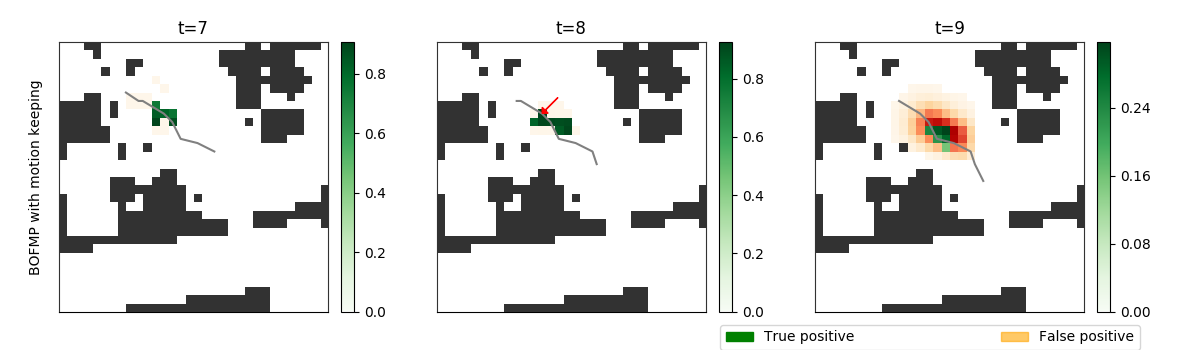
\includegraphics[width=\textwidth]{figures/moving_average_tracking.png}
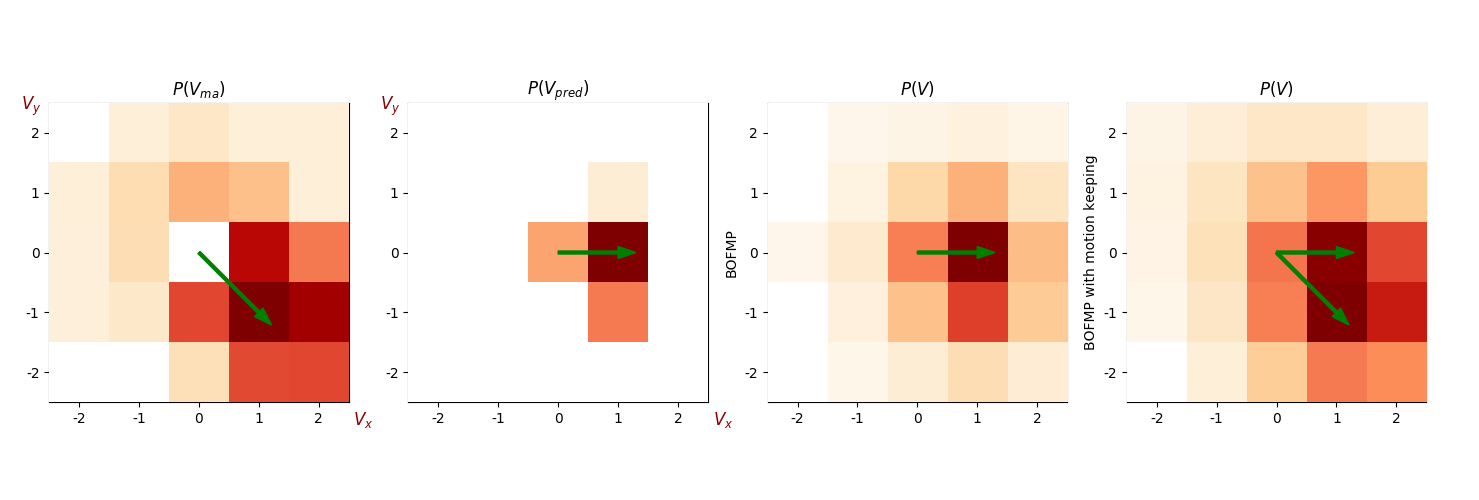
\includegraphics[width=\textwidth]{figures/moving_average_tracking_velocities_1.png}
\caption{\textbf{Up}: Three tracking steps of BOFMP with motion keeping. A person is walking from upper left towards lower right. The measurement is lost at $t=9$. \textbf{Down}: Velocities of the cell pointed by the red arrow at $t=8$. On each plot, the most possible direction is shown by green arrows. Based on measurements from $t=7$ and $t=8$, the predicted velocity $P(V_{pred})$ shows it is more likely the occupancy will propagates towards right for the next time step. However, the motion trend, which is represented by $P(V_{ma})$, shows it is more likely to move to lower right. As a consequence, BOFMP with motion keeping shows there are possibilities going both right and lower right, which is more realistic in this tracking example.}
\label{fig:keep_motion_idea}
\end{figure}


We randomly sample 100 sets of parameters for each scenario, evaluate them on training set, and select the best set of parameters based on the mean of average precisions for the future prediction stage ($t=9:16$). The best parameters are shown in Table \ref{table:best_param_real}.

\begin{table}[H]
\footnotesize
\centering  
\begin{tabularx}{\textwidth}{c|c|c|c|c|c|c|c|c|c}
    \hline
    & $ e $ & $ \delta^2 $ & $ \Omega $ & \sml{blurExt} & \sml{blurVar} & $w$ & \sml{initMF} & \sml{keepMF}  & \footnotesize{mean of a.p.}\\ \hline \hline
    BOFUM & 5 & 0.677 & 0.152  & - & - & - & - & - & 0.302   \\ \hline
    BOFMP & 5 & 0.649 & 0.191  & - & - & - & - & - & 0.321  \\
    \scriptsize{BOFMP spatial blurring} & 5 & 0.636 & 0.100  & 5 & 1.093 & - & - & - & 0.327  \\
    \scriptsize{BOFMP motion keeping} & 7 & 0.744 & 0.026  & - & - & 4 & 0.563 & 0.707 & 0.381  \\
   \hline
\end{tabularx}
\caption{Best parameters for BOFUM and BOFMP on real data.}
\label{table:best_param_real}
\end{table}

\normalsize
Then we apply each filter with its best parameters on test data of 244 scenes. Table \ref{table:real_test_data} lists the average precision in future prediction stage and their mean. Compared with BOFUM, our methods have performance gain of $29\%$, $31\%$ and $43\%$ respectively. Figure \ref{fig:real_test_data} shows the average precision for each time step. One can see that, as in the case of simulated data, average precision starts with values close to zero, and increase rapidly over the next two time steps. From $t=3$ to $t=8$, average precisions keep rather stable at high values, which proves that filters predict very well for the next immediate step. In future prediction stage ($t=9:16$), average precisions decrease severely as time horizon increases, since the state of the world becomes more uncertain. However, our BOFMP and its variants are still better than their baseline BOFUM for every time step in the future prediction stage.

\begin{table}[H]
\footnotesize
\centering  
\begin{tabularx}{.8\textwidth}{c|c|c}
    \hline
    & average precision for $t=9:16$ & mean \\ \hline \hline
    BOFUM & 0.670   0.512  0.384  0.314  0.252  0.205  0.167  0.148  & 0.331   \\ \hline
    BOFMP & 0.705  0.570   0.468  0.424  0.351  0.336  0.305  0.255 & 0.427  \\
    \scriptsize{BOFMP spatial blurring} & 0.694  0.564  0.480   0.439  0.371  0.349  0.311  0.264 &  0.434  \\
    \scriptsize{BOFMP motion keeping} &  0.762  0.675  0.561  0.496  0.405  0.353  0.305  0.238 & 0.474  \\
   \hline
  \end{tabularx}
\caption{Future predictions for BOFUM and BOFMP on real data.}
\label{table:real_test_data}
\end{table}
\normalsize

\begin{figure}[ht]
  \centering
   \captionsetup{width=\linewidth}
    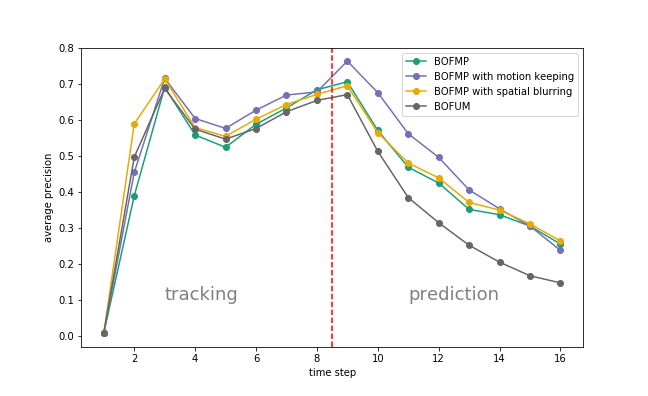
\includegraphics[width=.8\textwidth]{figures/test_on_real_data.png}
    \caption{Evaluation results on real test data. In the future prediction stage, our BOFMP and its variants are better than their baseline BOFUM for every time step, i.e., $t=9:16$.}
    \label{fig:real_test_data}
\end{figure}

\section{Applications}

\subsection{Future Occupancy Prediction}

Embedded with an accurate motion model of the tracking objects, our proposed BOFMP is able to predict reasonable occupancies even after a few time steps without measurements. This is demonstrated in Figure \ref{fig:idea}, where we show that our predictions on future occupancy outperform the baseline BOFUM. The accuracy of future occupancy prediction is critical in many applications, such as collision avoidance and path planing. Although our method of learning motion model is only demonstrated in the scenario of human tracking, it is applicable in other cases such as car tracking in ADAS systems. Therefore, our proposed method has huge potential in these applications. 

\begin{figure}[ht]
  \centering
    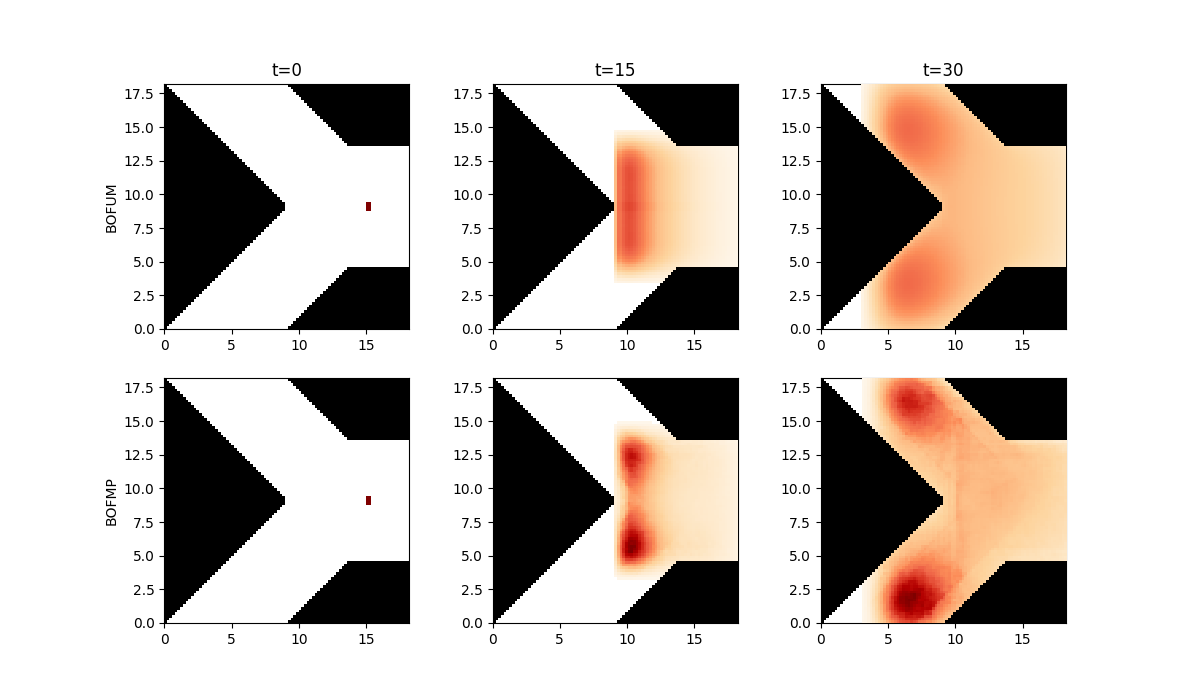
\includegraphics[width=\textwidth]{figures/idea.png}
    \caption{Occupancy predictions for BOFUM and our proposed BOFMP after several time steps without measurements. The map shows a Y-fork. At $t=0$, a person is shown as a red rectangle and with initial velocity towards left. At $t=15$, the person encounters intersection. BOFUM has no information about human motion pattern, and continues to propagate occupancy towards left. Our BOFMP knows that humans are likely to turn to either upper or lower corridors. At $t=30$, since occupancies going left vanish due to the wall, BOFUM predicts occupancies in corridors, but they are biased towards walls on the left. Our BOFMP predicts more occupancies in the middle of corridors, since it knows humans are more likely to walk in the middle.}
    \label{fig:idea}
\end{figure}

\subsection{Dynamic Analysis}
\subsection{Predict Occupied Area}

\begin{figure}[ht]
  \centering
    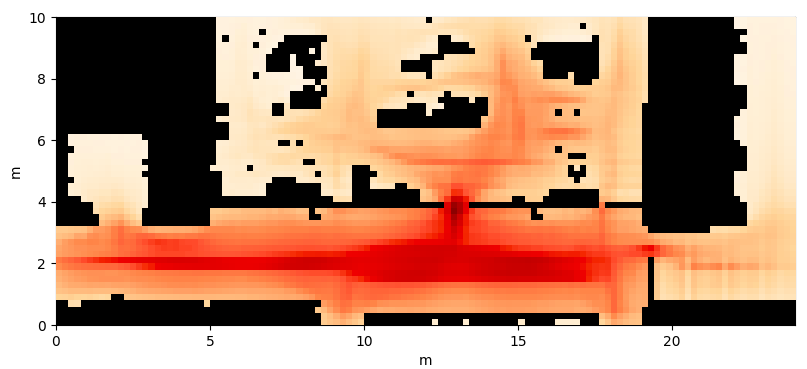
\includegraphics[width=\textwidth]{figures/average_occupancy_3.png} \\
    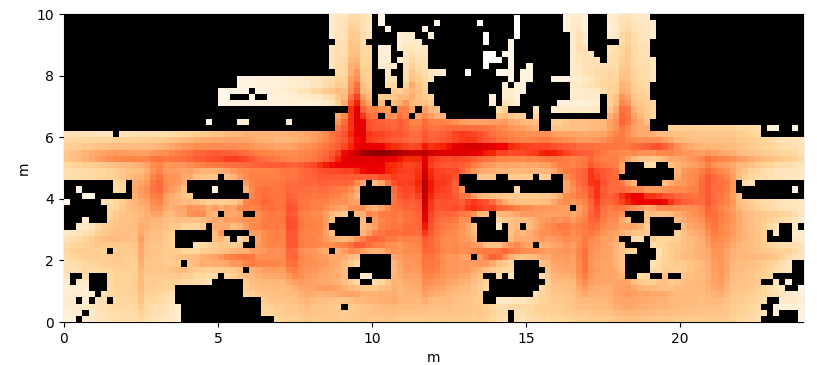
\includegraphics[width=\textwidth]{figures/average_occupancy_4.png} \\
    \caption[Average occupancy prediction on static map]{Average occupancy prediction on static map.} 
    \label{fig:average_occupancy_pred}
\end{figure}


 